\section{Risk preference changes the allocation tradeoff}\label{sec:15}

\begin{figure}[!htbp]\centering
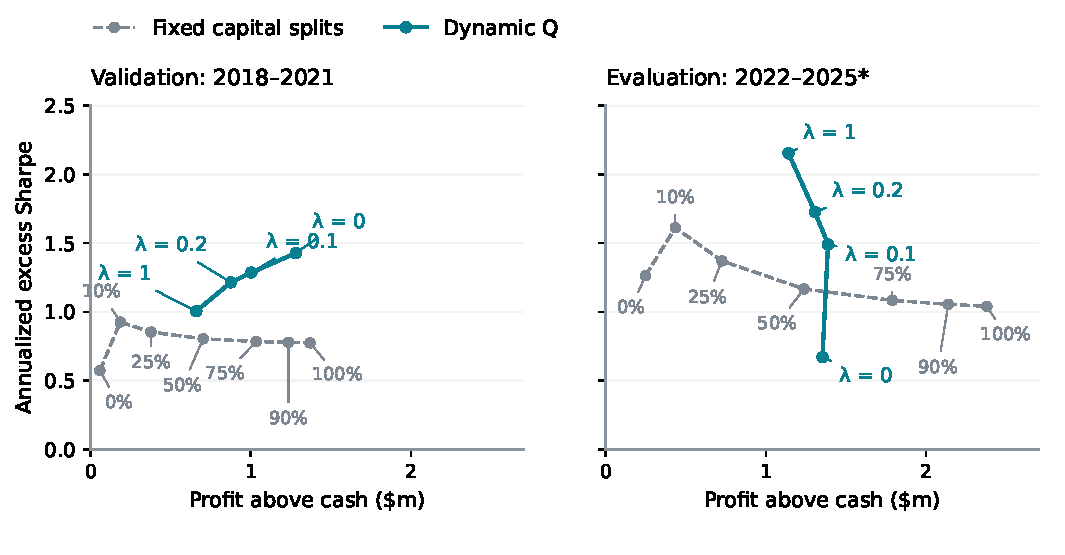
\includegraphics[width=\linewidth]{allocation_risk.pdf}
\caption{Bandit-managed source portfolios; nine-input Q state and \(\gamma\) = 0.99. Gray labels are fixed straddle percentages; the remainder goes to put pairs. Lines connect discrete policies. Both axes have the same scales across periods; 2025 ends in August.}\label{fig:allocation-risk}
\end{figure}

\begin{table}[H]\centering\small
\caption{Q-allocation outcomes under four reward preferences.}
\setlength{\tabcolsep}{4pt}\renewcommand{\arraystretch}{1.18}
\begin{tabularx}{\textwidth}{@{}>{\hsize=0.83008\hsize\linewidth=\hsize\raggedright\arraybackslash}X>{\hsize=0.99609\hsize\linewidth=\hsize\raggedleft\arraybackslash}X>{\hsize=1.02539\hsize\linewidth=\hsize\raggedleft\arraybackslash}X>{\hsize=1.07422\hsize\linewidth=\hsize\raggedleft\arraybackslash}X>{\hsize=1.07422\hsize\linewidth=\hsize\raggedleft\arraybackslash}X@{}}\toprule
\textbf{Reward} & \textbf{2018--21 S} & \textbf{2018--21 profit} & \textbf{2022--25 S} & \textbf{2022--25 profit}\\\midrule
\(\lambda\) = 0 & 1.427 & \$1.281m & 0.671 & \$1.353m\\
\(\lambda\) = 0.1 & 1.286 & \$1.003m & 1.491 & \$1.388m\\
\(\lambda\) = 0.2 & 1.215 & \$0.875m & 1.726 & \$1.306m\\
\(\lambda\) = 1 & 1.005 & \$0.660m & 2.152 & \$1.141m\\
\bottomrule\end{tabularx}\end{table}

With bandit entries and \(\lambda\) = 0.20, Q reaches later Sharpe 1.726 and \$1.306 million profit above cash. Fixed 50/50 gives 1.167 and \$1.238 million; the highest-Sharpe fixed split, 90/10, gives 1.612 and \$435,181. At \(\lambda\) = 1, Q trades some profit for Sharpe 2.152. Straddle-heavy fixed allocations still generate more dollars. The curve therefore describes a profit--risk tradeoff, not dominance on every objective. At \(\lambda\) = 0.20, annualized growth relative to cash is 2.34\% and excess volatility 1.35\%; at \(\lambda\) = 1 these are 2.13\% and 0.98\%.


At \(\lambda\) = 0, the learner aggressively pursues profit through the higher-dollar, higher-variance straddle strategy. It chooses straddles alone in 138 of 191 later decisions, with a mean straddle target of 73.2\%, versus 24.9\% at \(\lambda\) = 0.20 and 16.9\% at \(\lambda\) = 1. Validation Sharpe is 1.427, but later Sharpe falls to 0.671. When straddle performance weakens, this concentration becomes costly: the zero-penalty portfolio loses approximately \$331,000 above cash in 2025.


The problem also involves when capital is committed. A fixed 75\% allocation to straddles achieves later Sharpe 1.084, so average exposure alone does not explain the weaker Q result. The profit-only learner can respond to state, but its learned timing does not distinguish attractive straddle opportunities well enough in the later period. Positive penalties make large fluctuations costly and lead to more selective straddle exposure. Increasing Bellman updates from 200 to 500, 1,000 and 2,000 changes no later decision for these settings. This check points to the reward and learned allocation rule, rather than too few iterations.
